
\section{Measuring charge transport}

In this section the Hall measurement technique and analysis of the \BSCO samples is described. Transport measurements on superconductors have been performed for over a century now and was the technique by which superconductivity was first discovered. The relative technical simplicity of the measurements makes transport measurements highly appealing considering the wealth of information that can be extracted from a single curve.

The charge transport measurements performed for this thesis took place in Bristol in the Green `Polo' magnet for low fields and in the LNCMI pulsed field facility in Toulouse for the high field data. Also included is analysis of data taken by group members at the high field laboratory in Nijmegen, Netherlands. The six-probe measurement technique is the same for all the transport measurements with only slight adjustments between Hall and magnetoresistance measurements.

\subsection{Experimental apparatus}

\subsubsection{Six probe technique}

For accurate measurement of voltage, and hence resistance, across a sample, two wires are not sufficient. The wires themselves have a resistance and given that samples often have resistances in the region of a few Ohms this means that measurements would most be of electrical conduits rather than the sample. A solution to this problem is to instead supply the current for the voltage reading via one set of wires, and then take the voltage reading from another set meaning that a minimum of four wires and four contacts on the sample are required. To measure magnetoresistance we require the voltage wires to be placed upstream and downstream of the current, to measure the Hall effect we require the wires to be placed transverse to the current. Moreover it is useful to be able to take two transport measurements at a time so as to get an idea for the homogeneity of the sample and as well to provide some redundancy in case of breakage. Since the \BSCO samples that we studied were to have both measurements, six connection points were placed to each sample as shown in figure~\ref{Fig:Exp:BSCOSampleSchematic}.
\begin{figure}[htbp]
    \begin{center}
        \includegraphics[scale=0.9]{Chapter-ExperimentalTechnique/Figures/BSCOSampleSchematic/BSCOSampleSchematic}
        \caption{An example \BSCO crystal mounted on the quartz substrate. Voltage legs are labeled (a), (b), (c) and (d).}
        \label{Fig:Exp:BSCOSampleSchematic}
    \end{center}
\end{figure}
The connections were made with \unit{20}{\micro\metre} gold wire for the current and \unit{10}{\micro\metre} gold wire for the voltage leads and attached with DuPont 4929 conductive silver paint which dries at room temperature. As shown in the figure, the sample is raised from the quartz substrate so that when the temperature drops and the wires and sample thermally contract, there is some give so that the ensemble does not pull itself apart.

With the four voltage legs a variety of configurations can be achieved. Measuring across (a) and (b) is the magnetoresistance configuration, (a) and (c) is the Hall configuration. It is also possible to measure across (a) and (d) and provided the field is reversed from positive to negative, both the Hall and the magnetoresistance across the sample can be extracted.

Because the connections may not be exactly aligned and because the silver paint in practice tends to whet over the edge of the sample, magnetoresistance contributions may be found in the Hall configuration and vise-versa. For this reason it is generally advised to sweep both with a positive field to obtain $R_{\textrm{pos}}$ and a negative field to obtain $R_{\textrm{neg}}$ where $R$ is the resistance and separate the two out using,
\begin{align}
R_{\textrm{Hall}} &= \frac{1}{2}( R_{\textrm{pos}} - R_{\textrm{neg}} ) \\
R_{\textrm{MR}} &= \frac{1}{2}( R_{\textrm{pos}} + R_{\textrm{neg}} )
\end{align}


\subsubsection{Polo magnet}


The `Polo' magnet is an Oxford cryostat containing a \ac{VTI} refrigeration device that allows temperature from $\sim$\unit{1.4}{\kelvin} to room temperature to be achieved. The \ac{VTI} system is a vacuum sealed chamber in to which the sample probe is inserted and sealed at the top. This chamber is insulated from a bath of $^4$He in the main cryostat by a vacuum jacket. $^4$He is admitted into the \ac{VTI} chamber from the bath via an adjustable needle valve and is pumped through the chamber and over the sample by an external roughing pump. By almost closing off the needle valve entirely and applying a heater on the sample stage the full range of temperatures can be achieved. In practice, a couple of temperature ranges are defined which require different operational techniques and are specified in table~\ref{Table:Exp:PoloOperation}.
\begin{table}
    \begin{center}
           \caption{Operating the \ac{VTI} under various temperature regimes.}
        \begin{tabular}[htbp]{lp{7cm}}
\toprule
Temperature range & Practice \\
\midrule
\unit{1.4}{\kelvin} -- \unit{4.2}{\kelvin} & Fill \ac{VTI} chamber with helium, close off needle valve and adjust the pumping rate to tune the temperature. \\
\unit{4.2}{\kelvin} -- \unit{300}{\kelvin} & Empty the \ac{VTI} of helium and open the needle valve slightly, only pump a small amount and use the sample heater to set the temperature.  \\
\bottomrule
        \label{Table:Exp:PoloOperation}
        \end{tabular}
    \end{center}
\end{table}
The \ac{VTI} chamber itself has an electric heater which can be operated separately and is good for rapidly heating the system up to room temperature but is in general too course for measurements.

Heating is controlled by a Lakeshore 340 temperature controller with the sample stage heated from the heater output and the \ac{VTI} heater controlled from the analogue output which has been boosted via a custom built amplifier unit. Sample temperature is monitored by a Cernox mounted onto the sample stage and \ac{VTI} temperature from a thermometer mounted inside the \ac{VTI} chamber.

The sample stage can be rotated from an external stepper motor which is supplied from a custom power source. All the instruments mentioned are controlled from a custom PC running a Delphi program written by Dr. M. French which queues runs and records and displays data. Some calculation is performed inside of the software, however was not configured for these experiments. For this reason the angle and the current fields should be ignored and instead determined by hand.

For twin voltage measurements, two Stanford SR830 lock-in amplifiers were used with one supplying the current and measuring voltage and the second synchronised to the first and also measuring a voltage. The current supplied was supplied through a \unit{1}{\kilo\ohm} buffer resistor in order to approximate the supply to a current source\footnote{i.e. if ($R_{\textrm{sample}} + R_{\textrm{wires}}) << R_{\textrm{buffer}} $ at all $T$, then the current is given by $V_{\textrm{excitation}}/R_{\textrm{buffer}}$.}. The resulting voltages were passed through two passive Princeton Applied Research model 1900 low noise amplifiers set to $\times100$ before measurement although the actual amplification for typical resistances of $10$--$100\Omega$ at \unit{33}{\hertz} is $\times 98$.

\subsubsection{LNCMI Toulouse}

To access the normal state of the higher \Tc materials, we require fields larger than the \unit{13}{\tesla} available in the Polo at Bristol. For many of these cases we took measurements at the LNCMI pulsed field facility in Toulouse. Here large capaitor banks are discharged through liquid nitrogen cooled copper resistive magnets to achieve short (few tens of microseconds) but strong fields of up to \unit{60}{\tesla}. Pulses at the stronger end of the scale have more potential for damaging the magnet and take longer to cool down before the next pulse can be taken and so careful consideration is required to the type of pulse undertaken.

The results are recorded using a pair of Stanford SR830 lock-in amplifiers after passing through an active INA3 pre-amplifer set to a gain of $\times200$. The \emph{raw} signal for the pulse duration is recorded and the lock-in in algorithm is post-processed in software to avoid wasted pulses due to incorrect settings. The driving current is supplied by the lock-in amplifier and unless otherwise noted is \unit{5}{\volt} through a \unit{1}{\kilo\ohm} resistor giving a current source of \unit{5}{\milli\ampere}.

Cooling down to $\sim \unit{1.4}{\kelvin}$ is possible by pumping on the helium in the magnet bath. Higher temperatures could be achieved by pumping out the exchange gas and \TODO{Continue...}

\subsection{Sample size determination}

The length and the width of the samples were determined from calibrated optical microscope screen captures. The depth was determined post transport measurements with the help of Dr. Peter Heard using a \ac{FIB}. This images samples by rastering a focused beam of ions onto the sample surface and measuring the amount of ejected electrons or ions form the image. This process causes electrical charging of the surface which can in turn adversely affect the path of the highly focused incoming ions and so the sample to be imaged must be earthed in order to remain electrically neutral. For these samples, a line of 4929 silver paint was drawn between on of the contacts and the sample mounting puck.

\subsection{Data Analysis}

\subsubsection{Field lag correction}



